% The graph of the slide "E8: Event-based Interaction" in the Assignment 7 beamer deck
% (E7/beamer/deck.tex), without its PlugFest note. Built to SVG by make.sh.
\documentclass[border=3pt]{standalone}
\usepackage{tikz}
\usepackage{fontspec}
\setsansfont{GilliusADFNo2}[Path=../../assets/, Extension=.otf, UprightFont=*-Regular, BoldFont=*-Bold]
\renewcommand{\familydefault}{\sfdefault}
\usepackage{url}
\usetikzlibrary{arrows.meta}
\definecolor{HSGgreenDark}{HTML}{0A5F2D}
\begin{document}
% Scaled up so that the slide, which never enlarges a picture, can show it at full width.
\scalebox{2.5}{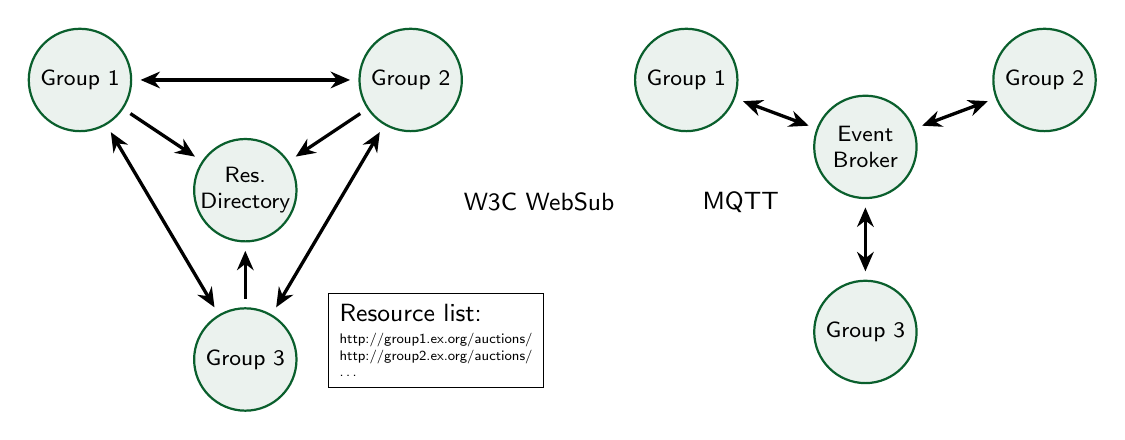
\begin{tikzpicture}[
    x=1cm, y=1cm,
    grp/.style={circle, draw=HSGgreenDark, fill=HSGgreenDark!8, thick,
                minimum size=1.3cm, inner sep=0pt, font=\footnotesize, align=center},
    >={Stealth[length=7pt, width=6pt]},
    link/.style={<->, very thick, shorten <=3pt, shorten >=3pt},
    uni/.style={->, very thick, shorten <=3pt, shorten >=3pt}]

  % W3C WebSub: every group subscribes to every other group; groups
  % register with the resource directory and share a resource list.
  \node[grp] (a1)  at (1.0,-0.75) {Group 1};
  \node[grp] (a2)  at (5.2,-0.75) {Group 2};
  \node[grp] (dir) at (3.1,-2.15) {Res.\\ Directory};
  \node[grp] (a3)  at (3.1,-4.3)  {Group 3};
  \draw[link] (a1) -- (a2);
  \draw[link] (a1) -- (a3);
  \draw[link] (a2) -- (a3);
  \draw[uni]  (a1) -- (dir);
  \draw[uni]  (a2) -- (dir);
  \draw[uni]  (a3) -- (dir);
  \node[draw, fill=white, anchor=north west, align=left, inner sep=4pt,
        font=\tiny] at (4.15,-3.45)
    {{\small Resource list:}\\[2pt]
     \url{http://group1.ex.org/auctions/}\\
     \url{http://group2.ex.org/auctions/}\\
     \ldots};
  \node[font=\small, anchor=west] at (5.75,-2.3) {W3C WebSub};

  % MQTT: hub-and-spoke via an event broker.
  \node[grp] (b1)  at (8.7,-0.75)   {Group 1};
  \node[grp] (b2)  at (13.25,-0.75) {Group 2};
  \node[grp] (brk) at (10.975,-1.6) {Event\\ Broker};
  \node[grp] (b3)  at (10.975,-3.95) {Group 3};
  \draw[link] (b1) -- (brk);
  \draw[link] (b2) -- (brk);
  \draw[link] (b3) -- (brk);
  \node[font=\small, anchor=east] at (10.0,-2.3) {MQTT};
\end{tikzpicture}}
\end{document}
